% Options for packages loaded elsewhere
\PassOptionsToPackage{unicode}{hyperref}
\PassOptionsToPackage{hyphens}{url}
\documentclass[
  ignorenonframetext,
]{beamer}
\newif\ifbibliography
\usepackage{pgfpages}
\setbeamertemplate{caption}[numbered]
\setbeamertemplate{caption label separator}{: }
\setbeamercolor{caption name}{fg=normal text.fg}
\beamertemplatenavigationsymbolsempty
% remove section numbering
\setbeamertemplate{part page}{
  \centering
  \begin{beamercolorbox}[sep=16pt,center]{part title}
    \usebeamerfont{part title}\insertpart\par
  \end{beamercolorbox}
}
\setbeamertemplate{section page}{
  \centering
  \begin{beamercolorbox}[sep=12pt,center]{section title}
    \usebeamerfont{section title}\insertsection\par
  \end{beamercolorbox}
}
\setbeamertemplate{subsection page}{
  \centering
  \begin{beamercolorbox}[sep=8pt,center]{subsection title}
    \usebeamerfont{subsection title}\insertsubsection\par
  \end{beamercolorbox}
}
% Prevent slide breaks in the middle of a paragraph
\widowpenalties 1 10000
\raggedbottom
\AtBeginPart{
  \frame{\partpage}
}
\AtBeginSection{
  \ifbibliography
  \else
    \frame{\sectionpage}
  \fi
}
\AtBeginSubsection{
  \frame{\subsectionpage}
}
\usepackage{iftex}
\ifPDFTeX
  \usepackage[T1]{fontenc}
  \usepackage[utf8]{inputenc}
  \usepackage{textcomp} % provide euro and other symbols
\else % if luatex or xetex
  \usepackage{unicode-math} % this also loads fontspec
  \defaultfontfeatures{Scale=MatchLowercase}
  \defaultfontfeatures[\rmfamily]{Ligatures=TeX,Scale=1}
\fi
\usepackage{lmodern}
\ifPDFTeX\else
  % xetex/luatex font selection
\fi
% Use upquote if available, for straight quotes in verbatim environments
\IfFileExists{upquote.sty}{\usepackage{upquote}}{}
\IfFileExists{microtype.sty}{% use microtype if available
  \usepackage[]{microtype}
  \UseMicrotypeSet[protrusion]{basicmath} % disable protrusion for tt fonts
}{}
\makeatletter
\@ifundefined{KOMAClassName}{% if non-KOMA class
  \IfFileExists{parskip.sty}{%
    \usepackage{parskip}
  }{% else
    \setlength{\parindent}{0pt}
    \setlength{\parskip}{6pt plus 2pt minus 1pt}}
}{% if KOMA class
  \KOMAoptions{parskip=half}}
\makeatother
\usepackage{color}
\usepackage{fancyvrb}
\newcommand{\VerbBar}{|}
\newcommand{\VERB}{\Verb[commandchars=\\\{\}]}
\DefineVerbatimEnvironment{Highlighting}{Verbatim}{commandchars=\\\{\}}
% Add ',fontsize=\small' for more characters per line
\newenvironment{Shaded}{}{}
\newcommand{\AlertTok}[1]{\textcolor[rgb]{1.00,0.00,0.00}{\textbf{#1}}}
\newcommand{\AnnotationTok}[1]{\textcolor[rgb]{0.38,0.63,0.69}{\textbf{\textit{#1}}}}
\newcommand{\AttributeTok}[1]{\textcolor[rgb]{0.49,0.56,0.16}{#1}}
\newcommand{\BaseNTok}[1]{\textcolor[rgb]{0.25,0.63,0.44}{#1}}
\newcommand{\BuiltInTok}[1]{\textcolor[rgb]{0.00,0.50,0.00}{#1}}
\newcommand{\CharTok}[1]{\textcolor[rgb]{0.25,0.44,0.63}{#1}}
\newcommand{\CommentTok}[1]{\textcolor[rgb]{0.38,0.63,0.69}{\textit{#1}}}
\newcommand{\CommentVarTok}[1]{\textcolor[rgb]{0.38,0.63,0.69}{\textbf{\textit{#1}}}}
\newcommand{\ConstantTok}[1]{\textcolor[rgb]{0.53,0.00,0.00}{#1}}
\newcommand{\ControlFlowTok}[1]{\textcolor[rgb]{0.00,0.44,0.13}{\textbf{#1}}}
\newcommand{\DataTypeTok}[1]{\textcolor[rgb]{0.56,0.13,0.00}{#1}}
\newcommand{\DecValTok}[1]{\textcolor[rgb]{0.25,0.63,0.44}{#1}}
\newcommand{\DocumentationTok}[1]{\textcolor[rgb]{0.73,0.13,0.13}{\textit{#1}}}
\newcommand{\ErrorTok}[1]{\textcolor[rgb]{1.00,0.00,0.00}{\textbf{#1}}}
\newcommand{\ExtensionTok}[1]{#1}
\newcommand{\FloatTok}[1]{\textcolor[rgb]{0.25,0.63,0.44}{#1}}
\newcommand{\FunctionTok}[1]{\textcolor[rgb]{0.02,0.16,0.49}{#1}}
\newcommand{\ImportTok}[1]{\textcolor[rgb]{0.00,0.50,0.00}{\textbf{#1}}}
\newcommand{\InformationTok}[1]{\textcolor[rgb]{0.38,0.63,0.69}{\textbf{\textit{#1}}}}
\newcommand{\KeywordTok}[1]{\textcolor[rgb]{0.00,0.44,0.13}{\textbf{#1}}}
\newcommand{\NormalTok}[1]{#1}
\newcommand{\OperatorTok}[1]{\textcolor[rgb]{0.40,0.40,0.40}{#1}}
\newcommand{\OtherTok}[1]{\textcolor[rgb]{0.00,0.44,0.13}{#1}}
\newcommand{\PreprocessorTok}[1]{\textcolor[rgb]{0.74,0.48,0.00}{#1}}
\newcommand{\RegionMarkerTok}[1]{#1}
\newcommand{\SpecialCharTok}[1]{\textcolor[rgb]{0.25,0.44,0.63}{#1}}
\newcommand{\SpecialStringTok}[1]{\textcolor[rgb]{0.73,0.40,0.53}{#1}}
\newcommand{\StringTok}[1]{\textcolor[rgb]{0.25,0.44,0.63}{#1}}
\newcommand{\VariableTok}[1]{\textcolor[rgb]{0.10,0.09,0.49}{#1}}
\newcommand{\VerbatimStringTok}[1]{\textcolor[rgb]{0.25,0.44,0.63}{#1}}
\newcommand{\WarningTok}[1]{\textcolor[rgb]{0.38,0.63,0.69}{\textbf{\textit{#1}}}}
\usepackage{graphicx}
\makeatletter
\newsavebox\pandoc@box
\newcommand*\pandocbounded[1]{% scales image to fit in text height/width
  \sbox\pandoc@box{#1}%
  \Gscale@div\@tempa{\textheight}{\dimexpr\ht\pandoc@box+\dp\pandoc@box\relax}%
  \Gscale@div\@tempb{\linewidth}{\wd\pandoc@box}%
  \ifdim\@tempb\p@<\@tempa\p@\let\@tempa\@tempb\fi% select the smaller of both
  \ifdim\@tempa\p@<\p@\scalebox{\@tempa}{\usebox\pandoc@box}%
  \else\usebox{\pandoc@box}%
  \fi%
}
% Set default figure placement to htbp
\def\fps@figure{htbp}
\makeatother
\setlength{\emergencystretch}{3em} % prevent overfull lines
\providecommand{\tightlist}{%
  \setlength{\itemsep}{0pt}\setlength{\parskip}{0pt}}
% Auto-generated by infrastructure/rendering/_pdf_latex_helpers.py::extract_math_font_preamble.
% Minimal header passed to Pandoc via -H so Beamer slides pick up the same math font
% as the combined-PDF path. Adjust the manuscript's preamble.md to change the font globally.
\usepackage{unicode-math}
\setmathfont{latinmodern-math.otf}
\usepackage{bookmark}
\IfFileExists{xurl.sty}{\usepackage{xurl}}{} % add URL line breaks if available
\urlstyle{same}
\hypersetup{
  hidelinks,
  pdfcreator={LaTeX via pandoc}}

\author{\texorpdfstring{}{}}
\date{}

\begin{document}

\section{Categorial Grammar: Syntax as Algebraic Composition and
Proof}\label{sec:categorial-grammar}

\begin{frame}[allowframebreaks]{Categorial Grammar: Syntax as Algebraic
Composition and Proof}
\textbf{Where we are in the argument.} \autoref{sec:case-categories}
built the case category --- a static snapshot of licensed role-to-role
morphisms. This chapter equips the framework with a \emph{compositional
syntax} on top of that static layer: Lambek pregroup types let each word
carry its own combinatory potential, and cup/cap contractions reduce a
parallel tensor of word-boxes to the single sentence type \(s\), so a
sentence becomes a proof of well-typedness rendered graphically as a
string diagram.
\end{frame}

\begin{frame}[allowframebreaks]{Each Word Is Its Own Grammar Rule}
\protect\phantomsection\label{each-word-is-its-own-grammar-rule}
Traditional generative grammar computes sentence structure using
top-down phrase-structure rules that recursively combine constituents.
Categorial grammar inverts this perspective: rather than specifying
abstract construction rules, it assigns each lexical item a dedicated
\emph{type} that encodes its combinatory potential. For example, a
transitive verb like ``chases'' is not loosely defined as ``a word
requiring a subject and object,'' but specifically assigned the
algebraic type \((n \backslash s) / n\)---an active function that
categorically demands a noun to its right (the object) and a noun to its
left (the subject) to yield a complete sentence.
\end{frame}

\begin{frame}[allowframebreaks]{Lambek's Residuation Law: Consuming and
Producing Types in Linear Order}
\protect\phantomsection\label{lambeks-residuation-law-consuming-and-producing-types-in-linear-order}
Lambek {[}-@lambek1958mathematics{]} laid the algebraic foundations by
introducing a \emph{residuated} structure on syntactic types. He defined
two binary operations---the left residual \(\backslash\) and the right
residual \(/\)---derived from the multiplicative connective \(\otimes\)
(concatenation). The fundamental axiom governing this system is the
residuation law:

\begin{equation}
A \otimes B \leq C \quad \iff \quad A \leq C / B \quad \iff \quad B \leq A \backslash C
\label{eq:eq-3-1}
\end{equation}

This law brilliantly captures the fundamental duality of syntax: a verb
of type \((n \backslash s) / n\) actively \emph{consumes} available noun
arguments to \emph{produce} a well-formed sentence. The resulting
\textbf{Lambek calculus} operates as a non-commutative intuitionistic
linear logic---non-commutative because strict word order dictates
meaning, and linear because the derivation logically consumes each
lexical resource exactly once.

\begin{block}{Pregroups Unlock Compact Closure: The Bridge to DisCoCat
String Diagrams}
\protect\phantomsection\label{pregroups-unlock-compact-closure-the-bridge-to-discocat-string-diagrams}
Lambek {[}-@lambek2004fine{]} later simplified the framework to
\textbf{pregroup grammars}, where each type \(a\) has a left adjoint
\(a^l\) and a right adjoint \(a^r\) satisfying:

\begin{equation}
a^l \cdot a \leq 1 \leq a \cdot a^l \qquad a \cdot a^r \leq 1 \leq a^r \cdot a
\label{eq:eq-3-2}
\end{equation}

Coecke, Sadrzadeh, and Clark revolutionized this formal structuralism in
2010 with the \textbf{DisCoCat} (Distributional Compositional
Categorical) model {[}-@coecke2010mathematical{]}. DisCoCat
mathematically unifies categorial grammar with distributional semantics
by defining strong monoidal functors mapping pregroup grammars directly
into vector spaces. As Duneau emphasizes, this approach ``allows the
meaning of a sentence to be computed as a function of both the
distributional meaning of the words involved, as well as its grammatical
form'' {[}-@duneau2021parsing{]}. By proving that pregroups and
finite-dimensional vector spaces both behave as rigid monoidal
categories, DisCoCat allows us to compute whole-sentence vector meanings
linearly from constituent word vectors.

In this system, grammaticality reduces to algebraic verification:
checking whether a sequence of types maps to the sentence type \(s\) via
\emph{contraction} (\(a^l \cdot a \to 1\)) and \emph{expansion}
(\(1 \to a \cdot a^l\)) operations. This reformulation unlocks the
DisCoCat framework (\autoref{sec:categorical-semantics}) because
pregroups function as \textbf{compact closed categories}, natively
supporting a computationally sound diagrammatic calculus. When a
derivation is ill-typed, contractions fail to close: there is no valid
reduction to \(s\). \autoref{sec:cognitive-security} develops the
security reading of that failure mode---typed interaction boundaries and
prompt injection as illicit role reassignment.
\end{block}
\end{frame}

\begin{frame}[fragile,allowframebreaks]{Cups, Caps, and Joyal--Street:
How Wires Prove Grammaticality}
\protect\phantomsection\label{cups-caps-and-joyalstreet-how-wires-prove-grammaticality}
The pivotal connection between categorial grammar and visualization
comes from Joyal and Street {[}-@joyalstreet1991geometry{]}, who proved
that morphisms in monoidal categories can be faithfully represented as
\emph{string diagrams}---planar graphs where:

\begin{itemize}
\tightlist
\item
  \textbf{Wires} represent types (objects of the category)
\item
  \textbf{Boxes} represent words or operations (morphisms)
\item
  \textbf{Vertical composition} represents sequential application
\item
  \textbf{Horizontal juxtaposition} represents the tensor product
  (concatenation)
\item
  \textbf{Cups and caps} represent the contraction/expansion of a
  pregroup
\end{itemize}

\autoref{fig:string-diagram} surveys three syntactic structures side by
side (progression from intransitive to passive);
\autoref{fig:native-discocat} shows the same transitive sentence
rendered by our native matplotlib pipeline---a direct computational
output confirming word-box layout, wire routing, and cup-contraction
geometry independently of DisCoPy; and
\autoref{fig:multilingual-isomorphism} demonstrates that type-logical
structure remains invariant across diverse surface word orders (SVO,
free, SOV).

\begin{figure}
\centering
\pandocbounded{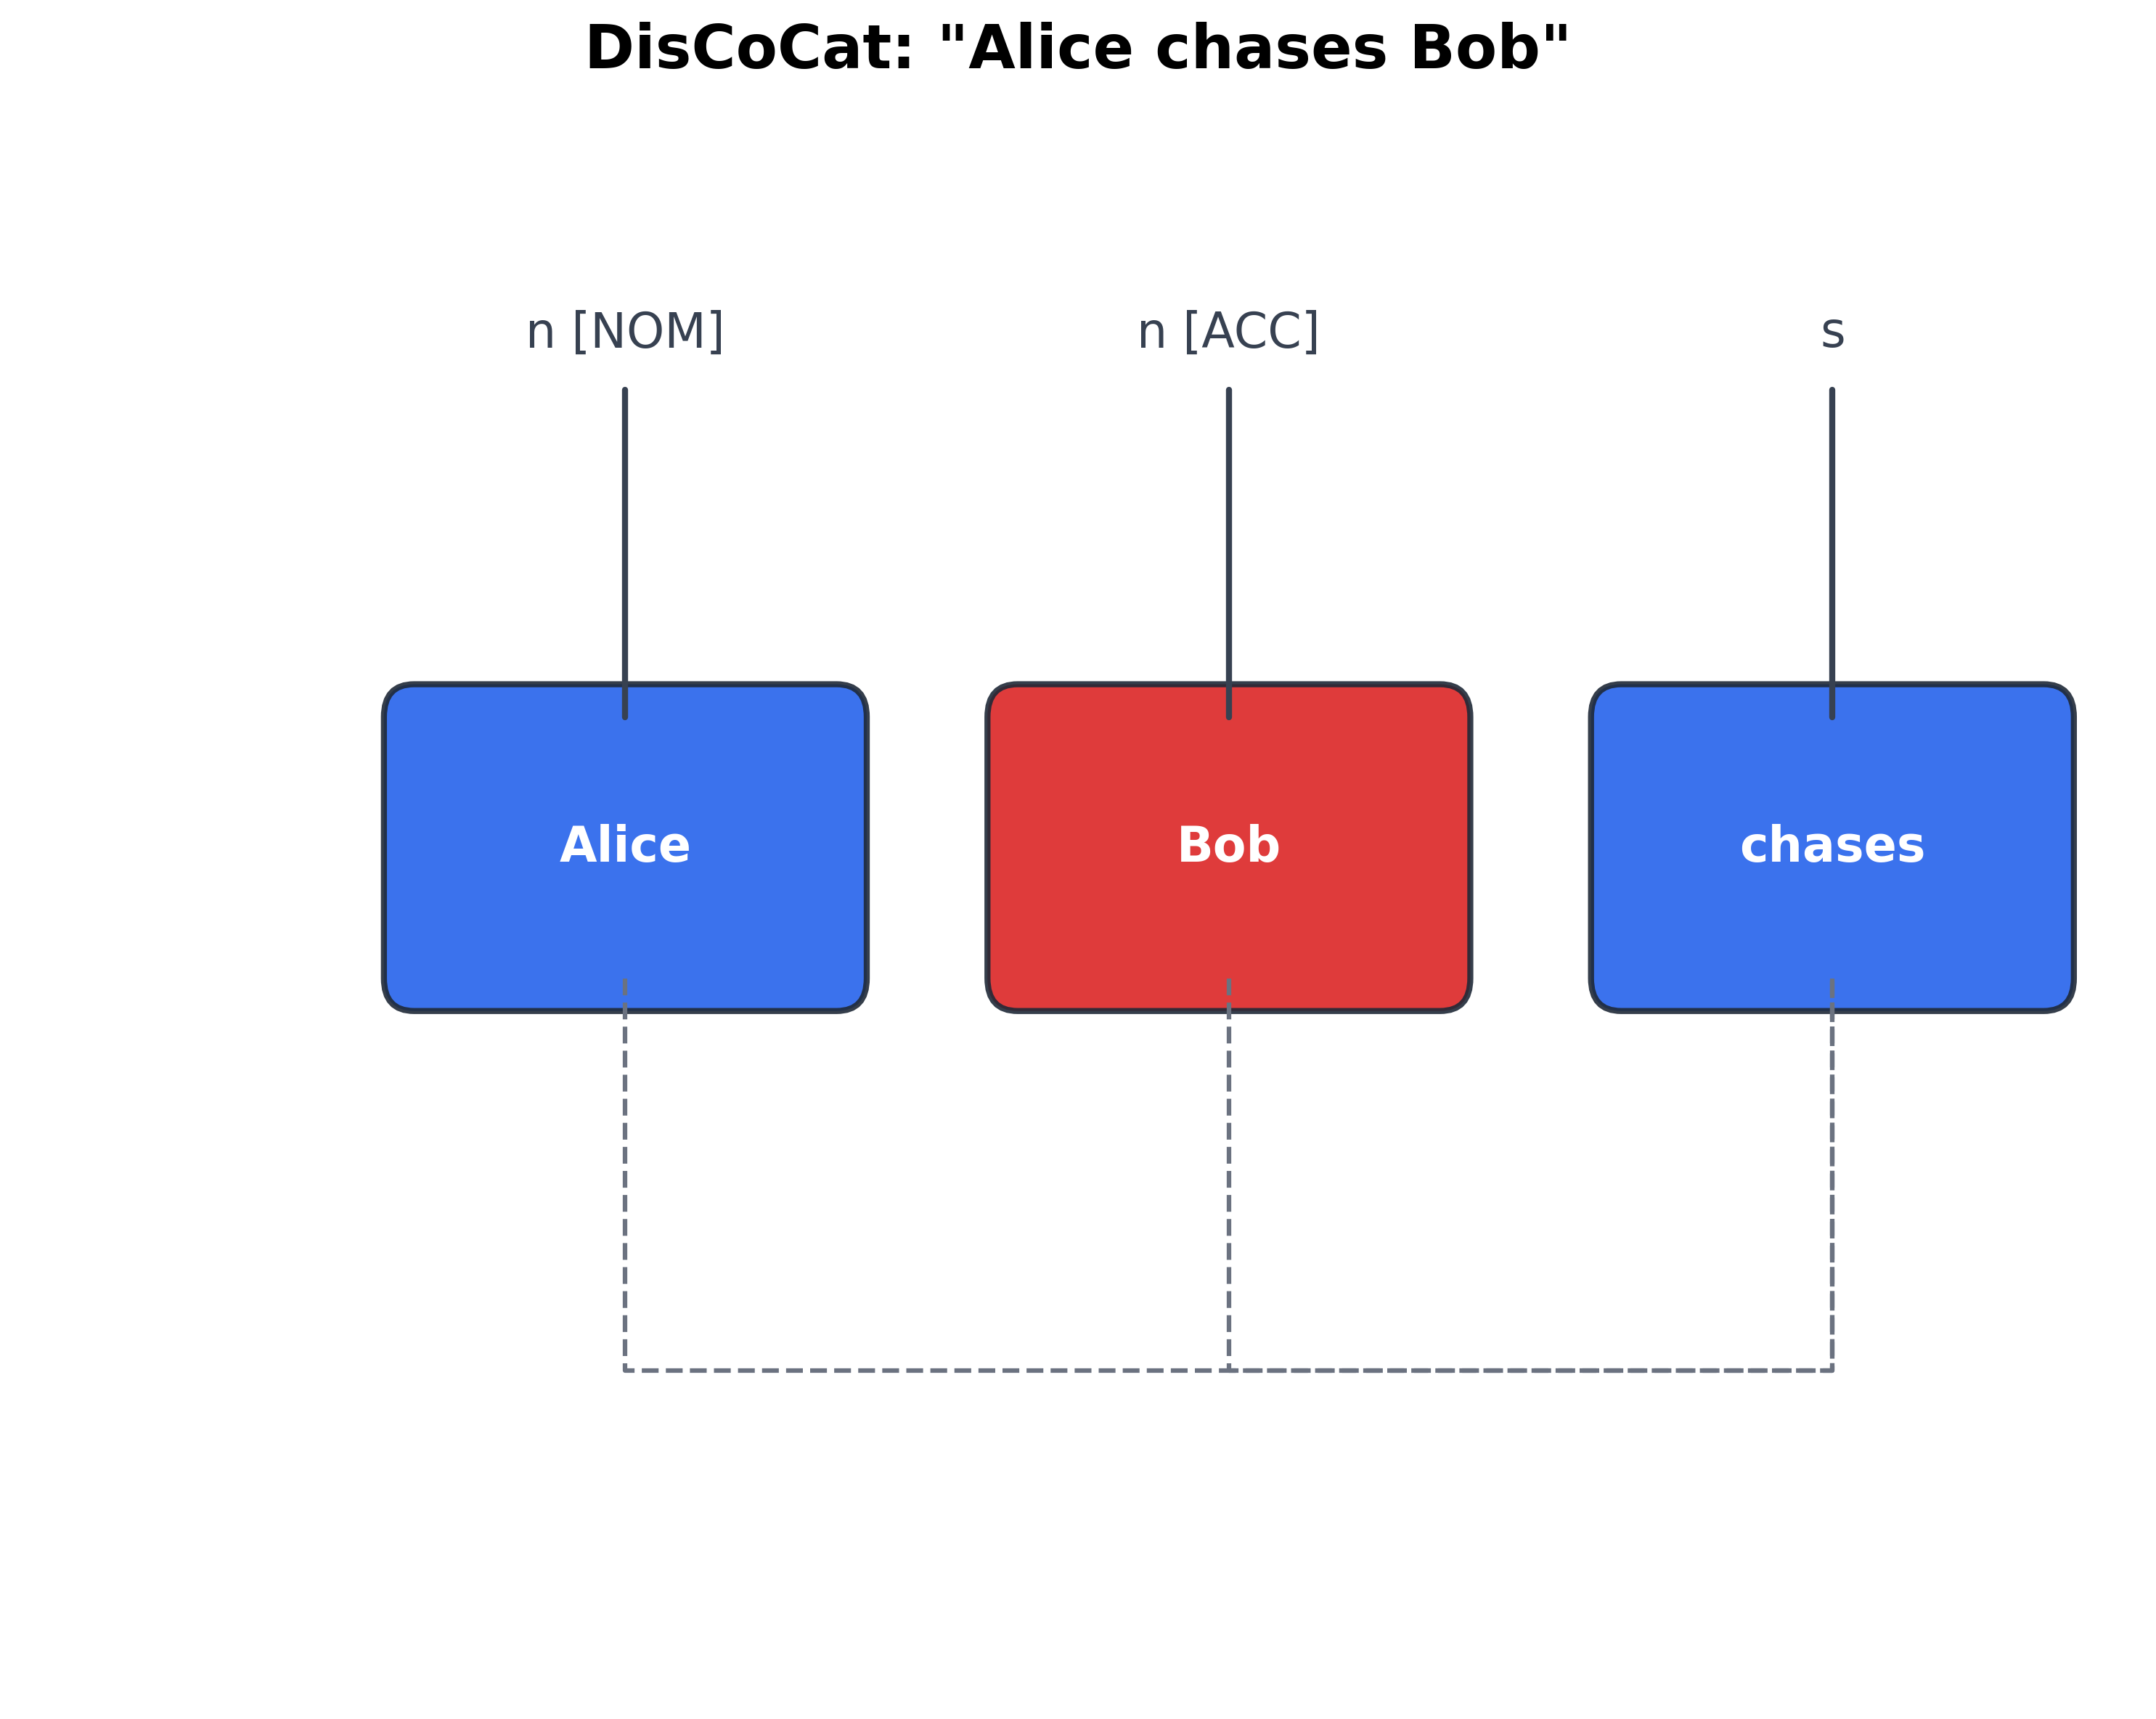
\includegraphics[keepaspectratio,alt={Native matplotlib rendering cross-validates DisCoPy pregroup geometry. String diagram for ``Alice chases Bob'' generated via src.visualization.string\_diagrams.render\_discocat\_sentence() without the DisCoPy library. Three Word boxes carry pregroup types: n (Alice, blue = NOM), n\^{}r \textbackslash otimes s \textbackslash otimes n\^{}l (chases, neutral), and n (Bob, red = ACC). Dashed arcs trace cup connections from noun wires to the verb's adjoint slots, rendering \textbackslash varepsilon: n\^{}r \textbackslash otimes n \textbackslash to 1 and \textbackslash varepsilon: n\^{}l \textbackslash otimes n \textbackslash to 1 as paired ligatures. This confirms that our visualization pipeline correctly reconstructs pregroup string-diagram geometry using only case-role metadata from src.case\_systems.case\_category, cross-validating the DisCoPy canonical output in .}]{../figures/string_diagram_discocat.png}}
\caption{Native matplotlib rendering cross-validates DisCoPy pregroup
geometry. String diagram for ``Alice chases Bob'' generated via
\protect\texttt{src.visualization.string\_diagrams.render\_discocat\_sentence()}
without the DisCoPy library. Three Word boxes carry pregroup types:
\(n\) (Alice, \textbf{blue} = NOM), \(n^r \otimes s \otimes n^l\)
(chases, \textbf{neutral}), and \(n\) (Bob, \textbf{red} = ACC). Dashed
arcs trace cup connections from noun wires to the verb's adjoint slots,
rendering \(\varepsilon: n^r \otimes n \to 1\) and
\(\varepsilon: n^l \otimes n \to 1\) as paired ligatures. This confirms
that our visualization pipeline correctly reconstructs pregroup
string-diagram geometry using only case-role metadata from
\protect\texttt{src.case\_systems.case\_category}, cross-validating the
DisCoPy canonical output in
\autoref{fig:discopy-transitive}.}\label{fig:native-discocat}
\end{figure}

\begin{figure}
\centering
\pandocbounded{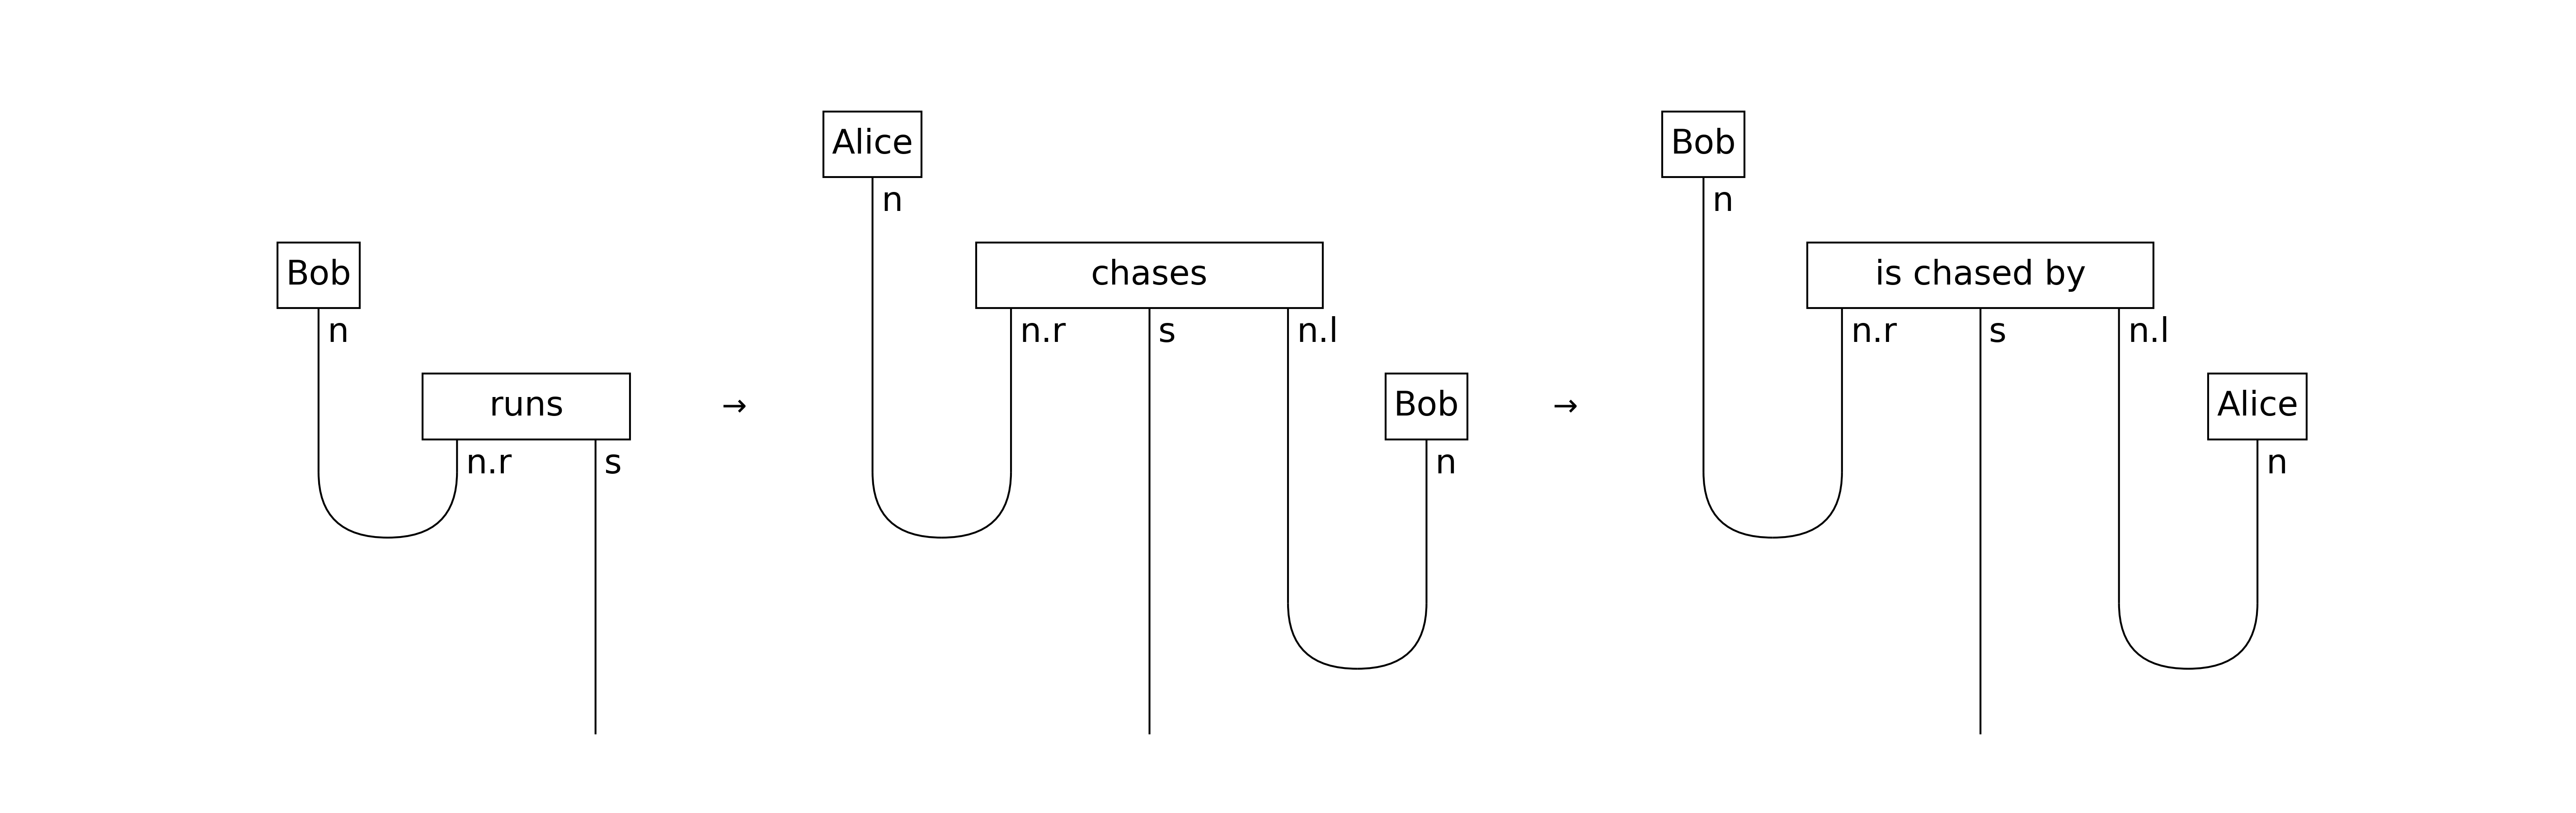
\includegraphics[keepaspectratio,alt={Valency determines diagram topology: Cup count tracks verb argument structure. A 1×3 DisCoPy pregroup grammar visualization of increasing argument complexity. Panel (a) intransitive ``Bob runs'' (NOM subject, 1 Cup contraction, type n \textbackslash otimes (n\^{}r \textbackslash otimes s) \textbackslash to s); Panel (b) transitive ``Alice chases Bob'' (NOM + ACC, 2 Cup contractions, type n \textbackslash otimes (n\^{}r \textbackslash otimes s \textbackslash otimes n\^{}l) \textbackslash otimes n \textbackslash to s); Panel (c) passive ``Bob is chased by Alice'' (patient promoted to NOM, former agent demoted to an oblique by-phrase; full transitive-shape verb type n\^{}r \textbackslash otimes s \textbackslash otimes n\^{}l with 2 Cup contractions --- which noun enters each cup is reversed relative to panel (b)). The role reassignment is visible as a topological swap of which noun lands in the left (subject) cup and which in the right (oblique) cup; cup count itself encodes argument-slot count, not syntactic prominence. Complexity metric \textbackslash kappa(D) per .}]{../figures/discopy_sentence_progression.png}}
\caption{Valency determines diagram topology: Cup count tracks verb
argument structure. A 1×3 DisCoPy pregroup grammar visualization of
increasing argument complexity. \textbf{Panel (a)} intransitive ``Bob
runs'' (NOM subject, 1 Cup contraction, type
\(n \otimes (n^r \otimes s) \to s\)); \textbf{Panel (b)} transitive
``Alice chases Bob'' (NOM + ACC, 2 Cup contractions, type
\(n \otimes (n^r \otimes s \otimes n^l) \otimes n \to s\));
\textbf{Panel (c)} passive ``Bob is chased by Alice'' (patient promoted
to NOM, former agent demoted to an oblique \emph{by}-phrase; full
transitive-shape verb type \(n^r \otimes s \otimes n^l\) with 2 Cup
contractions --- \emph{which} noun enters each cup is reversed relative
to panel (b)). The role reassignment is visible as a topological swap of
which noun lands in the left (subject) cup and which in the right
(oblique) cup; cup count itself encodes argument-slot count, not
syntactic prominence. Complexity metric \(\kappa(D)\) per
\autoref{eq:eq-4-4}.}\label{fig:string-diagram}
\end{figure}

\begin{figure}
\centering
\pandocbounded{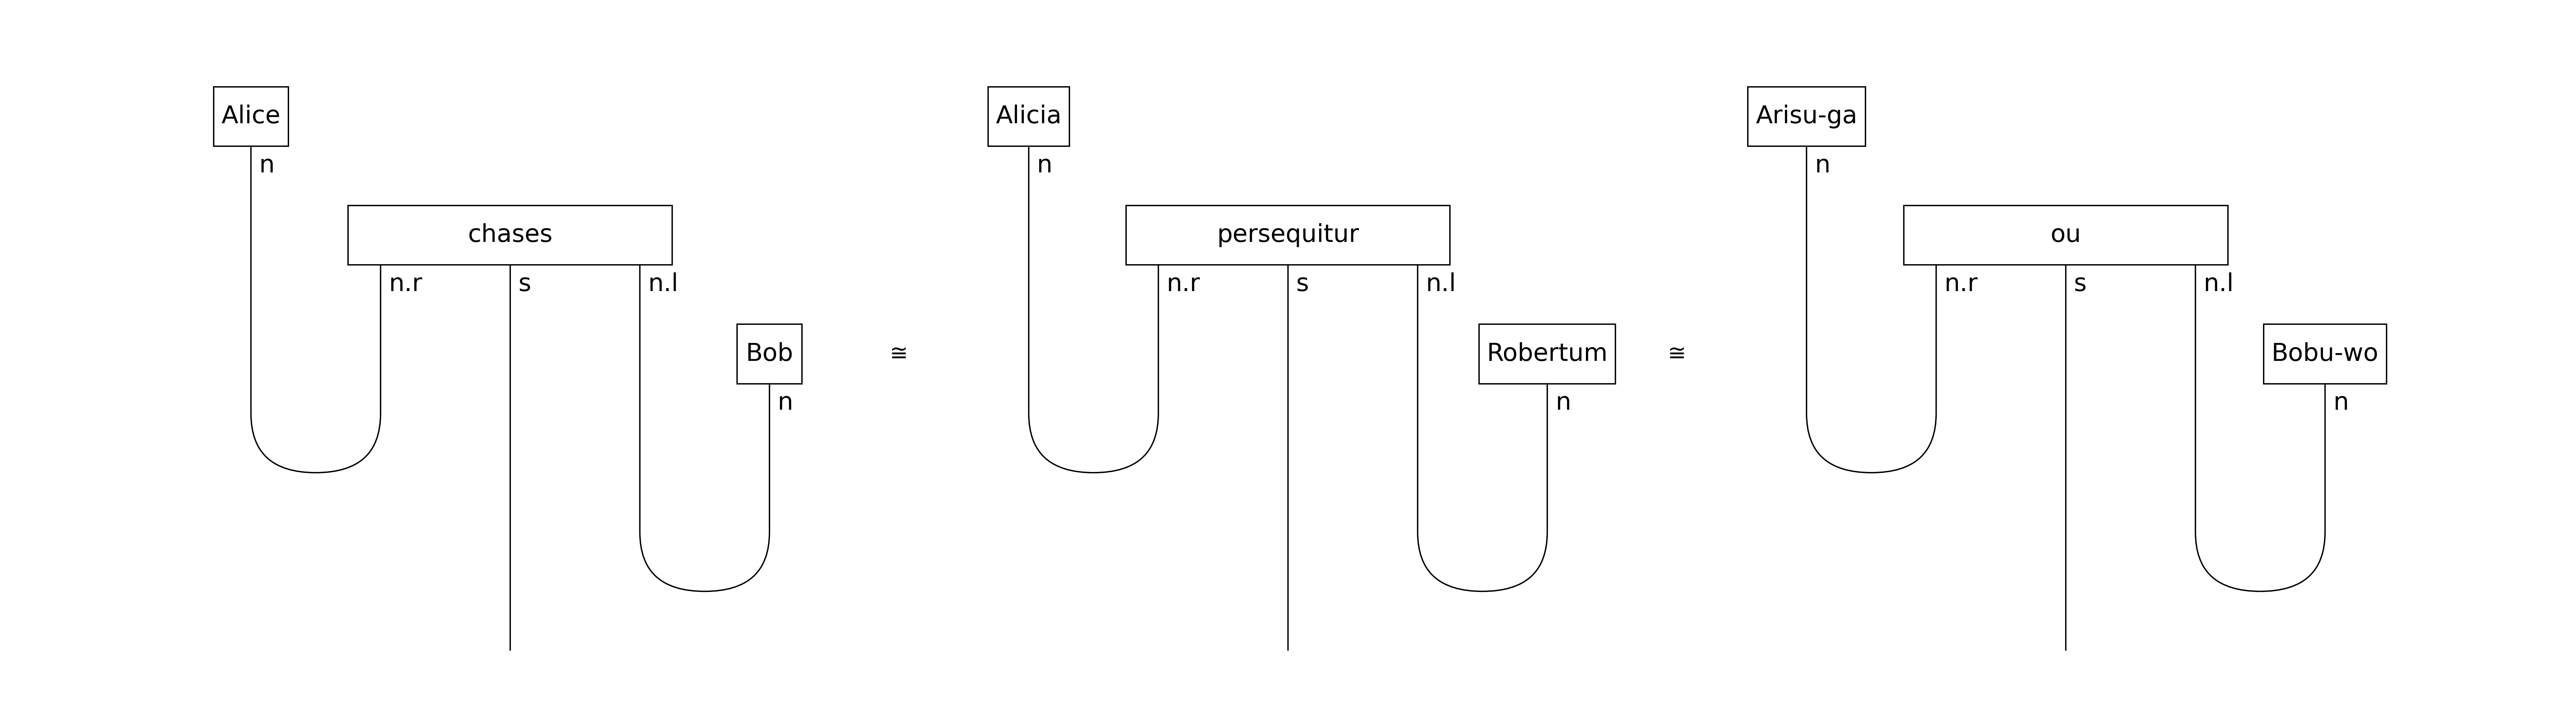
\includegraphics[keepaspectratio,alt={Type-logical structure is invariant under surface word-order permutation. Pregroup derivations for ``SUBJ chases OBJ'' across three typologically diverse languages: English (SVO), Latin (inflected, free order), and Japanese (agglutinative, SOV). Each renders an identical type reduction n \textbackslash otimes (n\^{}r \textbackslash otimes s \textbackslash otimes n\^{}l) \textbackslash otimes n \textbackslash to s, confirming the central claim of categorial grammar: syntactic universals reside in the type algebra, not in linear word order.}]{../figures/discopy_multilingual.png}}
\caption{Type-logical structure is invariant under surface word-order
permutation. Pregroup derivations for ``SUBJ chases OBJ'' across three
typologically diverse languages: English (SVO), Latin (inflected, free
order), and Japanese (agglutinative, SOV). Each renders an identical
type reduction
\(n \otimes (n^r \otimes s \otimes n^l) \otimes n \to s\), confirming
the central claim of categorial grammar: syntactic universals reside in
the type algebra, not in linear word
order.}\label{fig:multilingual-isomorphism}
\end{figure}

The Latin point in \autoref{fig:multilingual-isomorphism} generalises
directly to highly inflected modern Slavic. Russian \emph{Sobaka kusaet
čeloveka} ``the dog bites the man'' and its scrambled counterpart
\emph{Čeloveka kusaet sobaka} differ in linear order but share the
reduction
\(n_{\text{NOM}} \otimes (n^r \otimes s \otimes n^l) \otimes n_{\text{ACC}} \to s\),
with the case suffixes (-a NOM.SG.F vs -a ACC.SG.M.ANIM after stem
hardening) supplying the role information that English encodes
positionally. Serbian/BCS exhibits the same robustness: \emph{Pas ujeda
čoveka} / \emph{Čoveka ujeda pas} / \emph{Pas čoveka ujeda} (and three
further permutations) all type-check to \(s\) because the morphological
case marking on the noun wires uniquely identifies which is NOM and
which is ACC. In Slavic languages the type calculus is therefore not
just \emph{consistent} with the surface order --- the surface order is,
to a first approximation, \emph{immaterial}, with case morphology
carrying the entire wiring diagram explicitly.

This result---the soundness and completeness of string-diagrammatic
reasoning---formally guarantees that any topological conclusion drawn
visually from the diagram is algebraically valid: the diagram is not a
heuristic but a rigorous proof instrument.

This profound visual transparency instantiates exactly the ``free ride''
phenomenon identified by Shimojima {[}-@shimojima1996reasoning{]}: a
single diagram simultaneously exposes the syntactic derivation, the deep
argument structure, and the compositional flow of semantic
meaning---entirely eliminating the need for sequential, explicit
inference steps.

\textbf{Concrete derivation in DisCoPy.} The type reduction for ``Alice
chases Bob'' is computationally verified using the DisCoPy library's
\texttt{discopy.rigid} module:

\begin{Shaded}
\begin{Highlighting}[]
\ImportTok{from}\NormalTok{ discopy.rigid }\ImportTok{import}\NormalTok{ Ty, Box, Cup, Id}
\NormalTok{n, s }\OperatorTok{=}\NormalTok{ Ty(}\StringTok{\textquotesingle{}n\textquotesingle{}}\NormalTok{), Ty(}\StringTok{\textquotesingle{}s\textquotesingle{}}\NormalTok{)}
\NormalTok{alice }\OperatorTok{=}\NormalTok{ Box(}\StringTok{\textquotesingle{}Alice\textquotesingle{}}\NormalTok{, Ty(), n)}
\NormalTok{chases }\OperatorTok{=}\NormalTok{ Box(}\StringTok{\textquotesingle{}chases\textquotesingle{}}\NormalTok{, Ty(), n.r }\OperatorTok{@}\NormalTok{ s }\OperatorTok{@}\NormalTok{ n.l)}
\NormalTok{bob  }\OperatorTok{=}\NormalTok{ Box(}\StringTok{\textquotesingle{}Bob\textquotesingle{}}\NormalTok{,  Ty(), n)}
\NormalTok{words }\OperatorTok{=}\NormalTok{ alice }\OperatorTok{@}\NormalTok{ chases }\OperatorTok{@}\NormalTok{ bob          }\CommentTok{\# n ⊗ (n.r ⊗ s ⊗ n.l) ⊗ n}
\NormalTok{cups  }\OperatorTok{=}\NormalTok{ Cup(n, n.r) }\OperatorTok{@}\NormalTok{ Id(s) }\OperatorTok{@}\NormalTok{ Cup(n.l, n)}
\NormalTok{diagram }\OperatorTok{=}\NormalTok{ words }\OperatorTok{\textgreater{}\textgreater{}}\NormalTok{ cups               }\CommentTok{\# reduces to s}
\ControlFlowTok{assert}\NormalTok{ diagram.cod }\OperatorTok{==}\NormalTok{ s               }\CommentTok{\# type{-}checks: sentence type}
\end{Highlighting}
\end{Shaded}

The two \texttt{Cup} operations successfully contract \(n\) with \(n^r\)
(resolving the subject--verb link) and \(n^l\) with \(n\) (resolving the
verb--object link). This topological reduction collapses the five-wire
tensor product into a single, valid sentence wire \(s\). Consequently,
the assertion \texttt{diagram.cod\ ==\ s} constitutes a direct,
machine-processable proof of grammaticality.

\textbf{From pregroup types to graded types.} The standard pregroup
derivation produces a rigid, binary grammaticality judgment: the final
codomain of the fully contracted tensor product either matches the
sentence type \(s\) (grammatical) or fails (ill-formed). However, we can
\emph{grade} this binary verdict by replacing the underlying Boolean
algebra \(\{0,1\}\) with the continuous unit interval \([0,1]\). This
substitution yields a graded type theory where type judgments carry
continuous confidence weights rather than truth values. Asudeh and
Giorgolo {[}-@asudeh2020graded{]} developed this approach using a
monadic semantics that wraps base types inside a computational effect
tracking epistemic uncertainty---an idea whose categorical content is
precisely a change of enrichment base.

Mapped into our framework, this operation corresponds to the
\([0,1]\)-enrichment detailed in \autoref{sec:enriched-categories}: the
enriched scalar weight on any morphism \(f: A \to B\) quantifies the
confidence that the categorical case assignment \(A \to B\) remains
well-typed. From there, categorical magnitude aggregates these sparse,
local confidence scores into a global complexity measure evaluating the
entire syntactic derivation. The progression from rigid pregroup
strings, through graded types, into fully enriched case categories
operates mathematically as a cascade of base-change functors
(\(\mathbf{Bool} \hookrightarrow [0,1] \hookrightarrow \mathbf{R}_{\geq 0}\))---where
each successive level grants greater representational nuance while
demanding higher computational complexity.

\begin{figure}
\centering
\pandocbounded{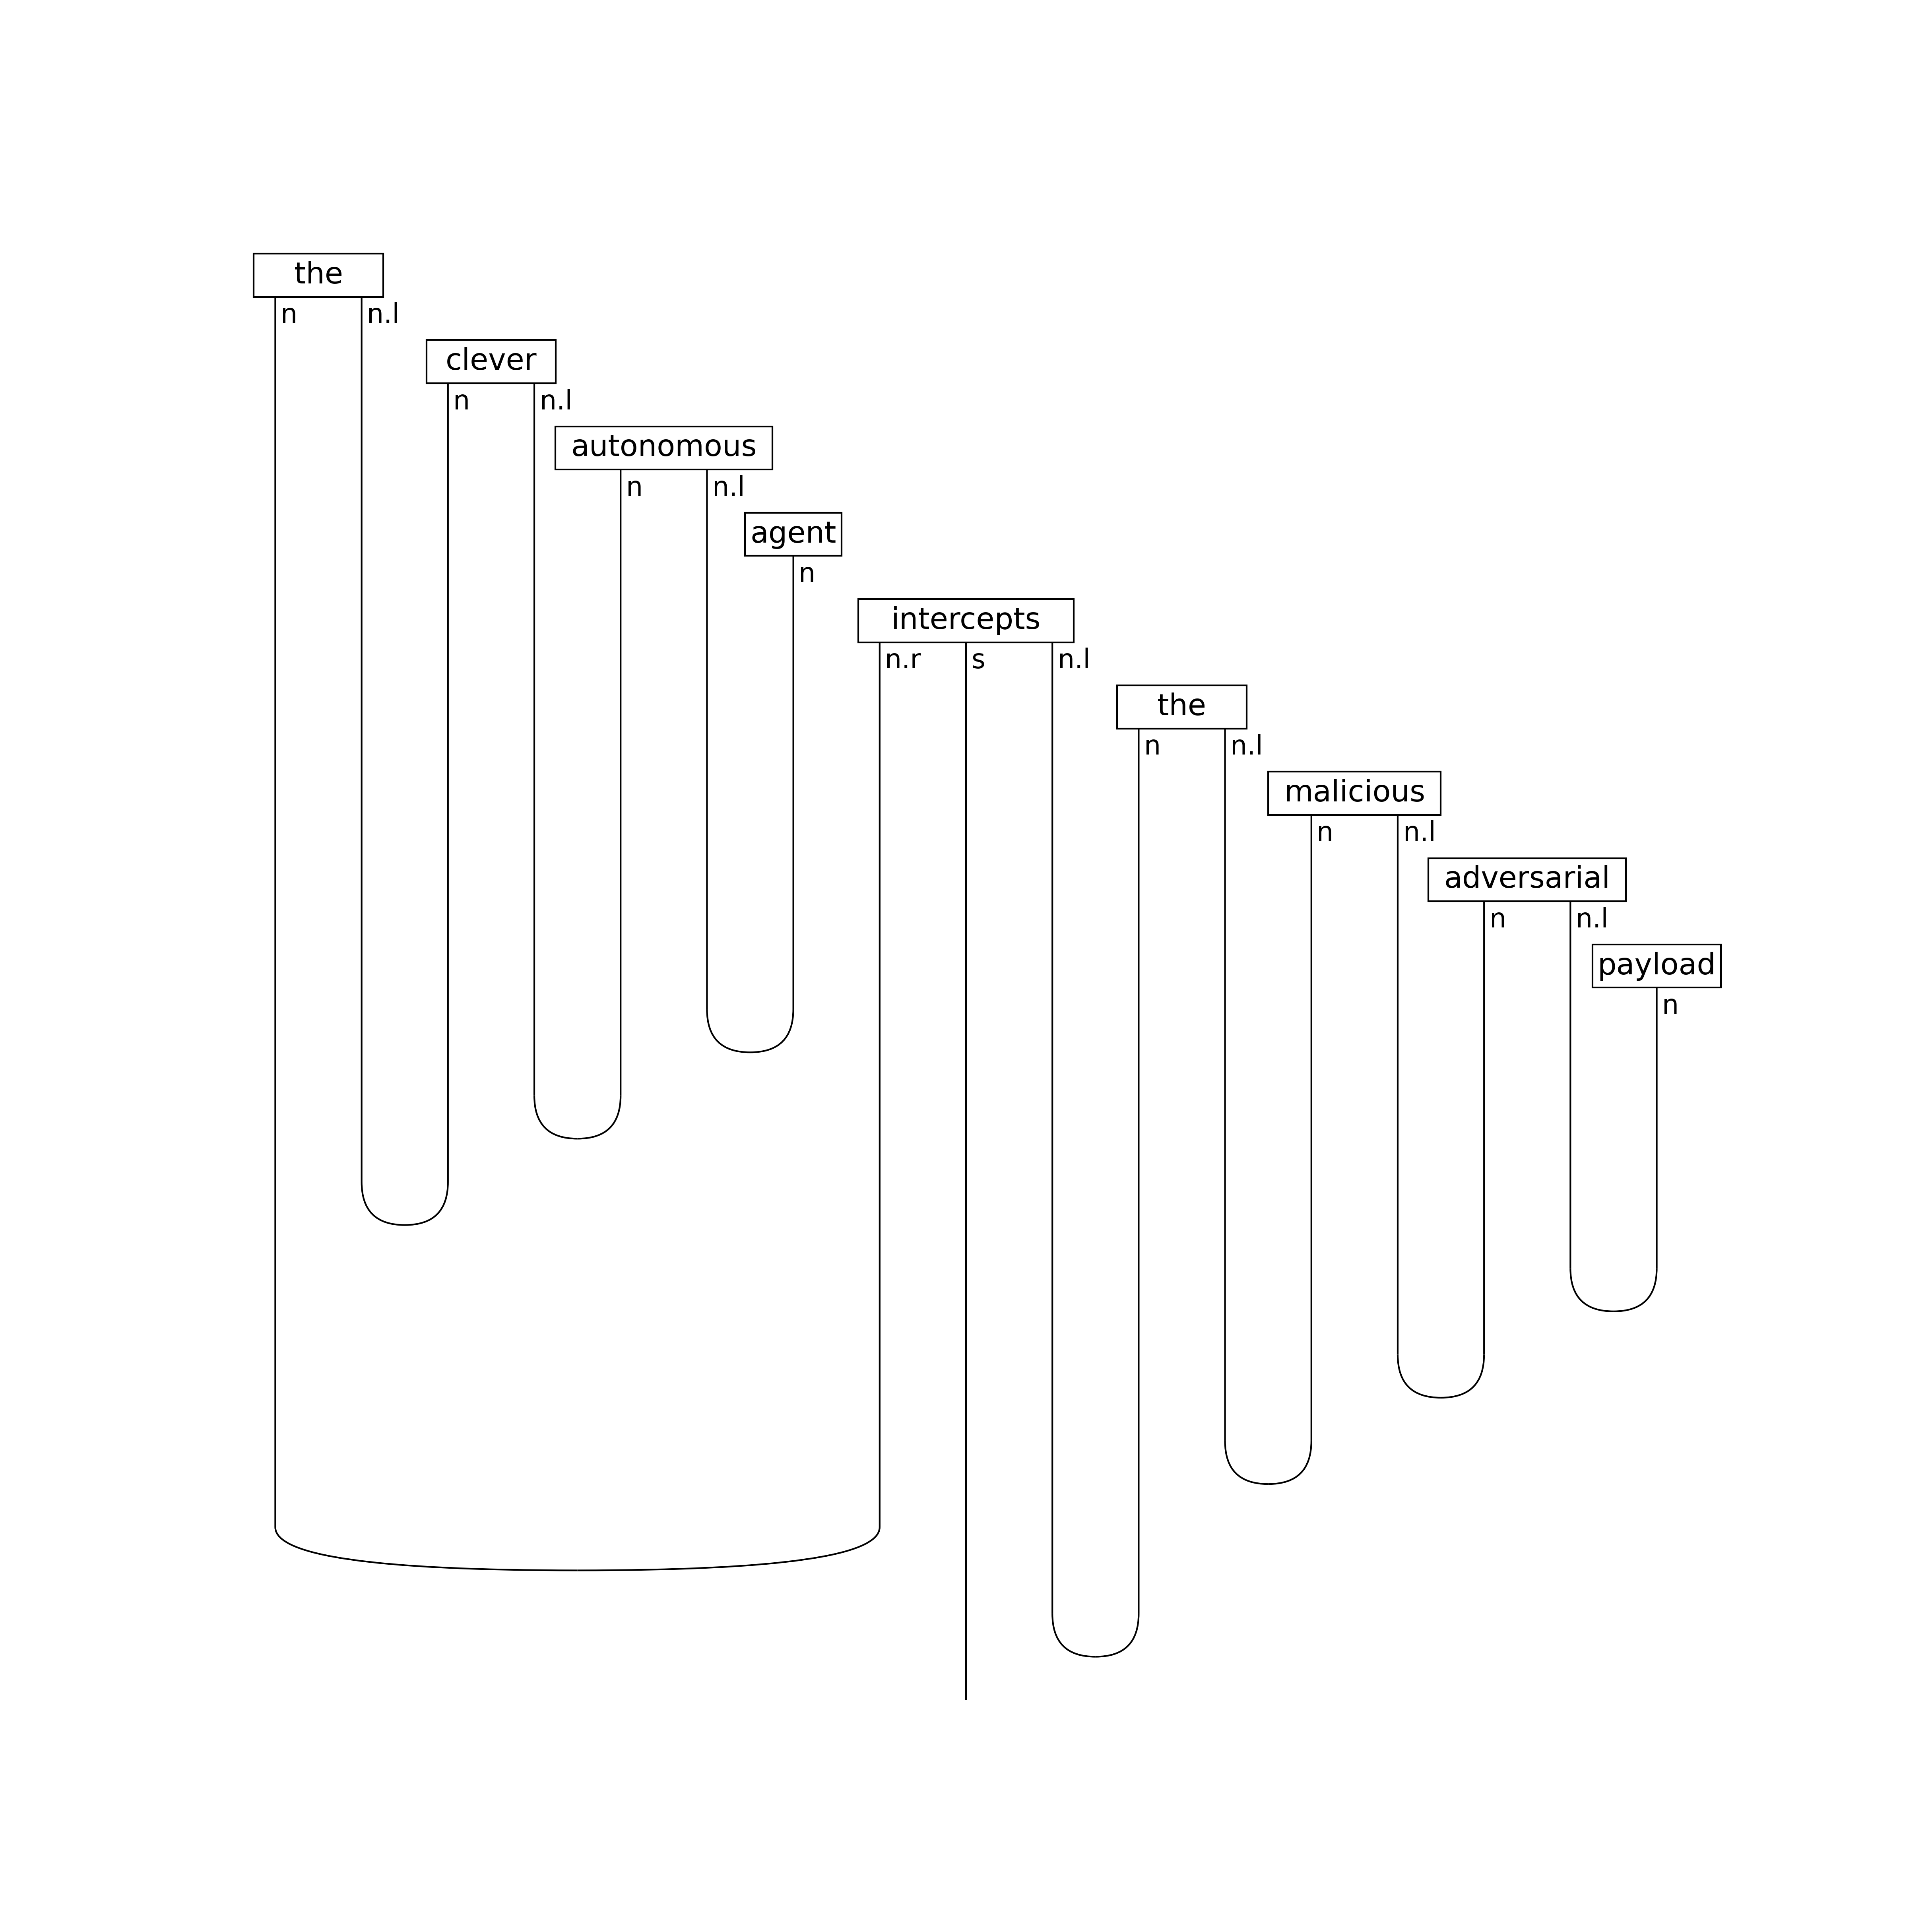
\includegraphics[keepaspectratio,alt={Direct DisCoPy machine output confirms pregroup type reduction to sentence wire s. Nine Word boxes carry complex noun-phrase types (e.g., n \textbackslash otimes n\^{}l for adjectives mapping an adjacent noun to a modified noun) and core verb types (n\^{}r \textbackslash otimes s \textbackslash otimes n\^{}l for the transitive ``intercepts''). Eight Cup contractions sequentially resolve the argument scopes from the deepest noun phrases outward, ultimately canceling all local adjoint pairs and reducing the extended initial tensor product to the single sentence wire s. Unlike the schematic progression in , this is the direct computational output of a multi-word discourse component, strictly confirming diagram.cod == s. By the Curry--Howard correspondence, this diagram simultaneously constitutes a syntactic derivation, a proof of well-typedness, and (under the meaning functor of ) a compositional semantic computation. Our extension decorates n-typed wires with functorial states S: \textbackslash mathbf\{Ent\} \textbackslash to \textbackslash mathbf\{Case\}, tracking role assignments across discourse boundaries via DisCoCirc entity wires.}]{../figures/discopy_transitive.png}}
\caption{Direct DisCoPy machine output confirms pregroup type reduction
to sentence wire \(s\). Nine Word boxes carry complex noun-phrase types
(e.g., \(n \otimes n^l\) for adjectives mapping an adjacent noun to a
modified noun) and core verb types (\(n^r \otimes s \otimes n^l\) for
the transitive ``intercepts''). Eight Cup contractions sequentially
resolve the argument scopes from the deepest noun phrases outward,
ultimately canceling all local adjoint pairs and reducing the extended
initial tensor product to the single sentence wire \(s\). Unlike the
schematic progression in \autoref{fig:string-diagram}, this is the
\emph{direct computational output} of a multi-word discourse component,
strictly confirming \protect\texttt{diagram.cod\ ==\ s}. By the
Curry--Howard correspondence, this diagram simultaneously constitutes a
syntactic derivation, a proof of well-typedness, and (under the meaning
functor of \autoref{sec:categorical-semantics}) a compositional semantic
computation. Our extension decorates \(n\)-typed wires with functorial
states \(S: \mathbf{Ent} \to \mathbf{Case}\), tracking role assignments
across discourse boundaries via \textbf{DisCoCirc entity
wires}.}\label{fig:discopy-transitive}
\end{figure}

For readers encountering pregroup reduction for the first time,
\autoref{fig:pregroup-unpacking} \emph{unpacks} the same construction
pedagogically: the four panels walk from the raw word types (panel 1),
through the parallel tensor that juxtaposes the boxes (panel 2), through
the application of the two cup contractions \(\varepsilon_n\) that
cancel each argument wire against its adjoint (panel 3), to the normal
form in which only the sentence wire \(s\) survives (panel 4). Each
panel is coloured by case role (NOM = blue, ACC = red, verb output in
indigo) so the identity of each wire is unambiguous.

\begin{figure}
\centering
\pandocbounded{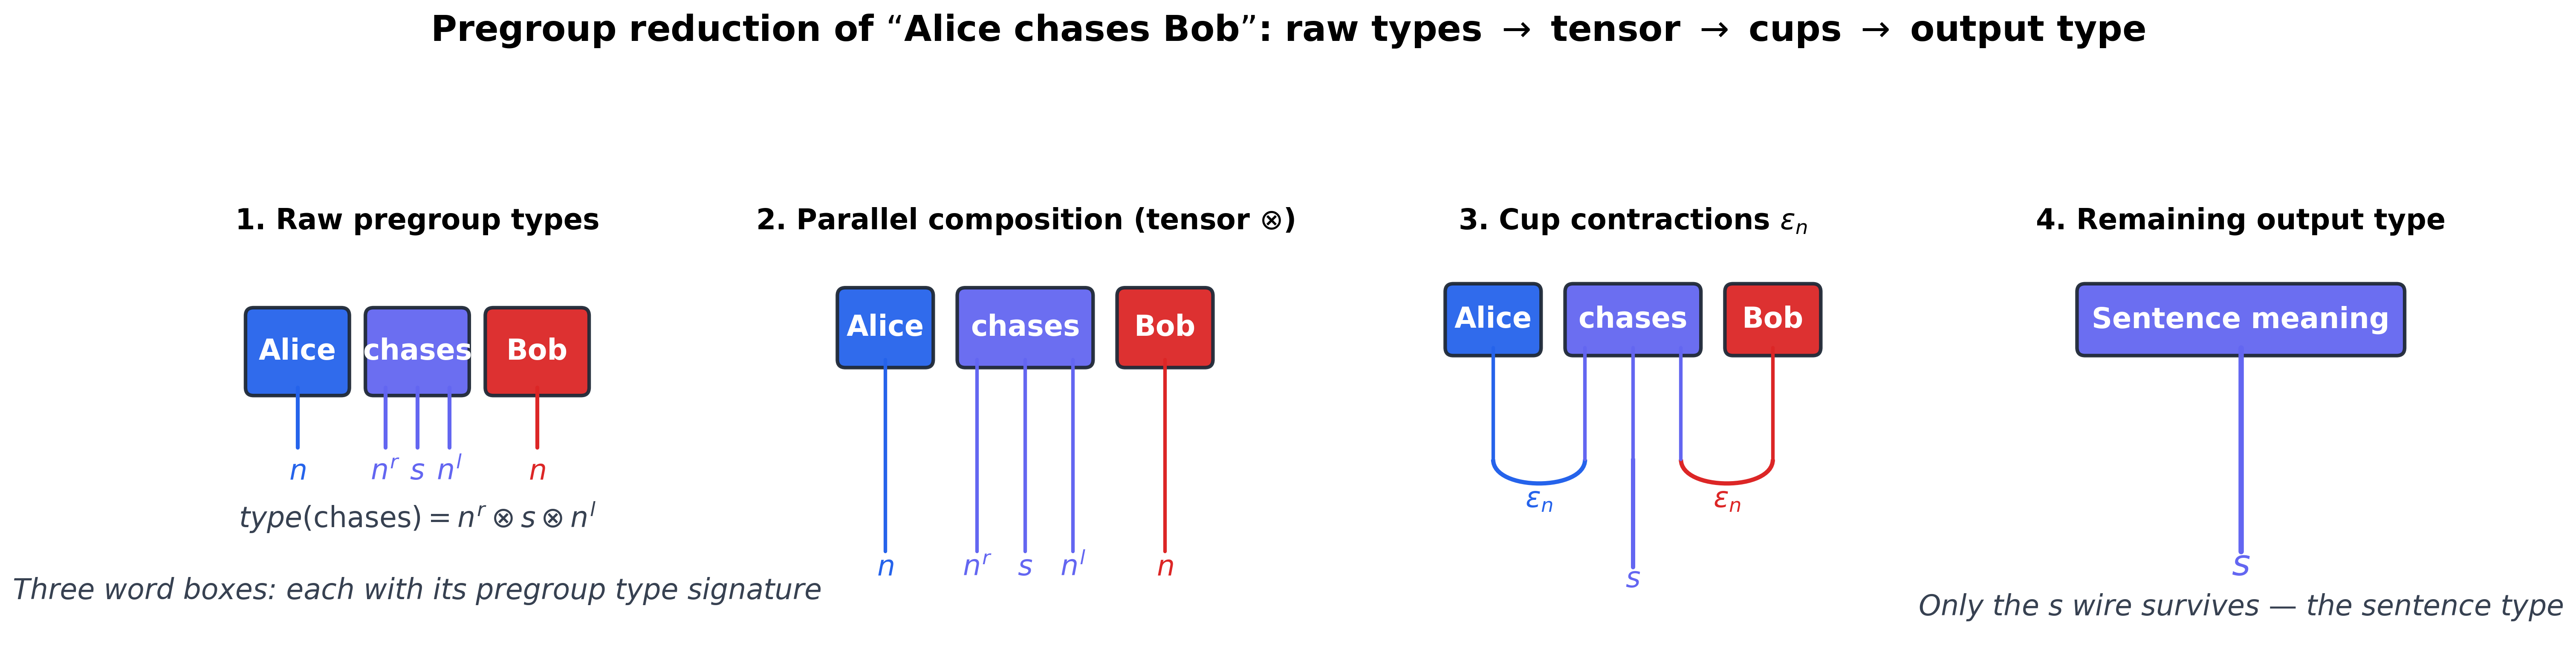
\includegraphics[keepaspectratio,alt={Pregroup reduction unpacked in four panels. Panel 1: raw pregroup types for Alice (n), chases (n\^{}r \textbackslash otimes s \textbackslash otimes n\^{}l), Bob (n). Panel 2: parallel composition \textbackslash otimes exposes all five dangling wires. Panel 3: the two cups \textbackslash varepsilon\_n cancel Alice's n against the verb's n\^{}r and the verb's n\^{}l against Bob's n, leaving only the central s wire. Panel 4: normal form --- the entire sentence reduces to a single s-typed wire. Generated programmatically from src.visualization.category\_unpacking.render\_pregroup\_reduction\_unpacking().}]{../figures/pregroup_reduction_unpacking.png}}
\caption{Pregroup reduction unpacked in four panels. Panel 1: raw
pregroup types for \emph{Alice} (\(n\)), \emph{chases}
(\(n^r \otimes s \otimes n^l\)), \emph{Bob} (\(n\)). Panel 2: parallel
composition \(\otimes\) exposes all five dangling wires. Panel 3: the
two cups \(\varepsilon_n\) cancel Alice's \(n\) against the verb's
\(n^r\) and the verb's \(n^l\) against Bob's \(n\), leaving only the
central \(s\) wire. Panel 4: normal form --- the entire sentence reduces
to a single \(s\)-typed wire. Generated programmatically from
\protect\texttt{src.visualization.category\_unpacking.render\_pregroup\_reduction\_unpacking()}.}\label{fig:pregroup-unpacking}
\end{figure}
\end{frame}

\end{document}
